\documentclass[a4paper]{article}

\usepackage{fullpage} % Package to use full page
\usepackage{parskip} % Package to tweak paragraph skipping
\usepackage{tikz} % Package for drawing
\usepackage{amsmath}
\usepackage{amsthm}
\usepackage{amsfonts}
\usepackage{hyperref}
\usepackage{enumitem}

\newcommand{\norm}[1]{\left\lVert#1\right\rVert}
\newcommand{\abs}[1]{\left\lvert#1\right\rvert}

\newtheorem{lemma}{Lemma}

\title{Data Mining: Homework 3}
\author{Anxhelo Xhebraj \\
        \href{mailto:xhebraj.1643777@studenti.uniroma1.it}{\texttt{xhebraj.1643777@studenti.uniroma1.it}}
        }
\date{ \{26 Nov .. 9 Dec\} 2018}

\begin{document}

\maketitle

\subsection*{Problem 2}

We will now study some questions of $k$-means on 1 dimension.

\begin{enumerate}
  \item Recall that in the $k$-means problem we want to minimize the total
    squared $\ell_2$ distance between each point and the center to which it is
    assigned to:
    \begin{align*}
      \sum_{i = 1}^{k} \sum_{x \in C_i} \norm{\mathbf{x} - \boldsymbol{\mu}_i}^2
    \end{align*}
    where $C_i$ is the set of points that belong to the $i$th cluster,
    $\boldsymbol{\mu}_i$ the mean of the points in the $i$th cluster, and
    \begin{align*}
      \norm{\mathbf{x}}^2 = \sum_{j = 1}^d x_j^2
    \end{align*}
    if $\mathbf{x} = (x_1, x_2, ..., x_d)$.

    In class, we said that in general the $k$-means problem is NP-hard. However,
    for $d$ = 1 the problem is polynomial. Design an algorithm that solves the
    $k$-means problem in time polynomial in the number of points $n$ and the
    number of clusters $k$, for $d$ = 1.

    (\textbf{Hint}: Can you solve the problem for $k$ clusters if you assume
    that you can solve it for fewer than $k$ clusters?)

    \textbf{Solution}: Let $X \subset \mathbb{R}, |X| = n$ be the set of points we want
    to cluster and denote by $\mathbf{x} = (x_1, x_2, ..., x_n)$ the sequence of
    elements in $X$ sorted by value and let $\mathbf{x}[i:j] = (x_i, x_{i + 1}, ..., x_{j}) $.
    The problem of $k$-means for $d = 1$ can be rewritten as finding $k$ indices
    $i_1, i_2, ..., i_k$ that minimize
    \begin{align*}
      \sum_{j = 0}^{k - 1} \phi(\mathbf{x}[i_j:i_{j + 1}]), \qquad \text{with } i_0 =
      1
    \end{align*}

    where $\phi(\mathbf{y}), \mathbf{y} = (y_1, y_2, ..., y_m)$ is the
    contribute to the $k$-means cost of a sequence of points, i.e.
    
    \begin{align*}
      \phi(\mathbf{y}) &= \sum_{i = 1}^m \abs{y_i - \mu(\mathbf{y})}^2 \\
      \mu(\mathbf{y}) &= \frac{\sum_{i = 1}^m y_i}{m}.
    \end{align*}

    Note that this is equivalent to finding $k$ partitions that minimize the
    cost however we reduce the set of possible partitions to
    
    \begin{align*}
      \mathcal{P}(X) = \{P = (P_1, P_2, ..., P_k) | x_i
    \in P_o \land x_j \in P_o \land x_i < x_l < x_j \implies x_l \in P_o\}
    \end{align*}

    i.e. intervals of the $\mathbb{R}$ space.


    \begin{lemma}
      Let $P = (P_1, P_2, ..., P_k)$ be the optimal solution to the $k$-means
      problem for set $X = \{x_1, x_2, ..., x_n\}$ and let $x_i \in P_o$ and $x_j
      \in P_o$ with $x_i \neq x_j$. For any $x \in X$ such that $x_i < x <
      x_j$ then $x \in P_o$.
    \end{lemma}
    \begin{proof}
      Assume by contradiction $x \in P_p \neq P_o$. Given that $P$ is optimal
      then
      \begin{align*}
        \abs{x - \mu(P_p)}^2 < \abs{x - \mu(P_o)}^2
      \end{align*}
      Without loss of generality assume $x \geq \mu(P_o)$ then we have the
      following cases:
      \begin{enumerate}
        \item $\mu(P_o) < \mu(P_p) < x$: this would cotradict the hypothesis
          since by
        attaching $x_j$ to $P_p$ would lower the cost which by hyp was optimal.

        \item $ x < \mu(P_p) < x + \abs{x - \mu(P_o)} $ again assigning $x_j$ to
          $P_p$ would lower the cost contradicting the optimality hypothesis.
      \end{enumerate}
      The same holds for $x \le \mu(P_o)$ with $x_i$.
    \end{proof}
\end{enumerate}

    \iffalse
    \begin{figure}[!htbp]
    \begin{center}
    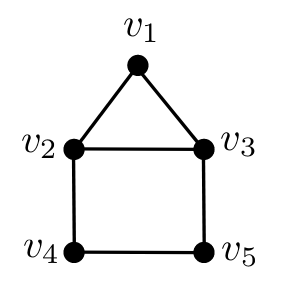
\includegraphics[width=70pt]{house.png}
    \end{center}
    \caption{\textit{The house subgraph}}\label{house}
    \end{figure}
    \fi

\end{document}
